
\section{ Introduction to OSM}
\begin{figure}[ht]
	\centering 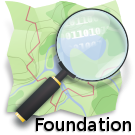
\includegraphics[scale=.50]{input/images/osm-logo.png}
	\caption{OSM foundation}
\end{figure}

  OpenStreetMap (OSM) is a collaborative project to create a free editable map of the world. The creation and growth of OSM has been motivated by restrictions on use or availability of map information across much of the world, and the advent of inexpensive portable satellite navigation devices. OSM is considered a prominent example of volunteered geographic information.\\

Created by Steve Coast in the UK in 2004, it was inspired by the success of Wikipedia and the predominance of proprietary map data in the UK and elsewhere. Since then, it has grown to over 2 million registered users, who can collect data using manual survey, GPS devices, aerial photography, and other free sources. This crowdsourced data is then made available under the Open Database Licence. The site is supported by the OpenStreetMap Foundation, a non-profit organisation registered in England and Wales.\\

Rather than the map itself, the data generated by the OpenStreetMap project is considered its primary output. The data is then available for use in both traditional applications, like its usage by Craigslist, OsmAnd, Geocaching, MapQuest Open, JMP statistical software, and Foursquare to replace Google Maps, and more unusual roles like replacing the default data included with GPS receivers. OpenStreetMap data has been favourably compared with proprietary datasources, though data quality varies worldwide.\\
 
\textbf{Map usage}
Map is available on the following platform.
\begin{itemize}
\item \textbf{Web browser}
    Data provided by the OpenStreetMap project can be viewed in a web browser with JavaScript support via Hypertext Transfer Protocol (HTTP) on its official website.\\
\item \textbf{OsmAnd}
    OsmAnd is free software for Android and iOS mobile devices that can use offline vector data from OSM. It also supports layering OSM vector data with prerendered raster map tiles from OpenStreetMap and other sources.\\
\item \textbf{Maps.me}
    Maps.me is free software for Android and iOS mobile devices that provides offline maps based on OSM data.\\
\item \textbf{GNOME Maps}
    GNOME Maps is a graphical front-end written in JavaScript and introduced in GNOME 3.10. It provides a mechanism to find the user's location with the help of GeoClue, finds directions via GraphHopper and it can deliver a list as answer to queries.\\
\item \textbf{Marble}
    Marble is a KDE virtual globe application which received support for OpenStreetMap.\\
\item \textbf{FoxtrotGPS}
    FoxtrotGPS is a GTK+-based map viewer, that is especially suited to touch input. It is available in the SHR or Debian repositories.\\
\item \textbf{Emerillon}
    Another GTK+-based map viewer.\\

\item The web site OpenStreetMap.org provides a slippy map interface based on the Leaflet JavaScript library (and formerly built on OpenLayers), displaying map tiles rendered by the Mapnik rendering engine, and tiles from other sources including OpenCycleMap.org.\\

\item Custom maps can also be generated from OSM data through various software including Jawg Maps, Mapnik, Mapbox Studio, Mapzen's Tangrams.\\

\item OpenStreetMap maintains lists of online and offline routing engines available, such as the Open Source Routing Machine. OSM data is popular with routing researchers, and is also available to open-source projects and companies to build routing applications (or for any other purpose).\\
\end{itemize}

